\chapter{MCL Sequencer:}
MCL features a powerful sequencer. There are 16 step sequencer tracks dedicated to the MD and 6 polyphonic tracks dedicated to External Midi devices, each has track independent length and playback speed.
\section{MD Sequencer Tracks:}
\begin{itemize}
\item 16 Track Sequencer with 64 max steps per track.
\item Conditional Trigs, Slide, Mute and Micro Timing per step.
\item 8 lockable parameters per track with 256 locks available per track.
\item Trigless Locks.
\item Real time record for both step and lock data.
\item Chromatic Mode.
\item Arpeggiator.
\end{itemize}
\section{External MIDI Sequencer tracks:}
\begin{itemize}
\item There are 6 x Ext MIDI Sequencer Tracks.
\item Each External MIDI track can be used to sequence an attached MIDI device on port 2. This could be an Elektron Analog 4, Elektron Monomachine or a generic MIDI device such as a synth module.
\item
    Features of the new Ext MIDI Sequencer:
\begin{itemize}
    \item 6 x Tracks
    \item 128 steps per track
	\item 512 events per track.
    \item A maximum of 16 events per step, (i.e 16 note polyphony)
	\item Each event could be an automation parameter or note on/off message.
    \item Microtiming per event
    \item Conditional trig per event
    \item Velocity per step
    \item Each track includes 8 MIDI Control Channel automation parameters with optional slide (linear interpolation).
    \item ProgramChange as CC destination.
    \item Arpeggiator.
\end{itemize}

\section{Auxiliary tracks:}
There are four auxiliary track types
 \begin{itemize}
 \item \textbf{MDFXTrack (FX):} Store and recall MachinDrum MasterFX settings: Delay, Reverb, EQ, Dynamics.
 \item \textbf{LFOTrack (LF):} Store and recall LFO page settings.
 \item \textbf{RouteTrack (RT):} Store and recall MD Track Routing and Chromatic Mode's Poly settings.
 \item \textbf{TempoTrack (TP):} Store and recall Tempo.

 
    \end{itemize}
\end{itemize}
\chapter{Sequencer: Saving and Loading}

Depending upon the track type, sequencer tracks are saved to or loaded from specific slots on either Grid X or Grid Y. 

\begin{itemize}
    \item 16 x MD Sequencer tracks are stored/loaded from slots 0 to 15 in Grid X, they correspond to MD tracks 1-16.
    \item 6 x External MIDI Sequencer tracks are stored/loaded from slots 0 to 5 in Grid Y. If the Analog4 was attached these would correspond to A4 tracks 1- 4, with 2 spare tracks for general MIDI.
    \item 4 x Auxiliary tracks are stored/loaded from slots 12 to 15 in Grid Y. 
\end{itemize}

\textit{Saving and Loading slots is accomplished through the use of the Save and Load pages and is described in the next chapter(s).}\\

Loaded tracks can be edited via their respective editor. The Step Edit page is used to edit MD sequencer tracks whilst the PianoRoll Editor is used to edit External MIDI Sequencer tracks.\\

When loading tracks, the internal sequencer data will be loaded from the slot and placed in the corresponding sequencer track. The slot's sound data is then transmitted to the corresponding track on the attached MIDI device. If the sequencer is stopped this occurs immediately, if the sequencer is running, then loading occurs according to behaviour described in the chapter "Chain Mode".\\

When saving to a slot, the corresponding internal sequencer track's data is stored, if the slot is mapped to a MIDI device such as the MD, the sound data of the corresponding track is retrieved from the device and also saved.\\
\\
\textit{Pattern/step sequencer data from an Elektron device is not retained. However, for the Machinedrum, the Save page offers the possibility of copying the corresponding MD track's pattern data to the slot's internal sequencer data via the options "MD", or "MERGE" (see next chapter, Save Page)}
\\\\

\begin{figure}
    \centering
    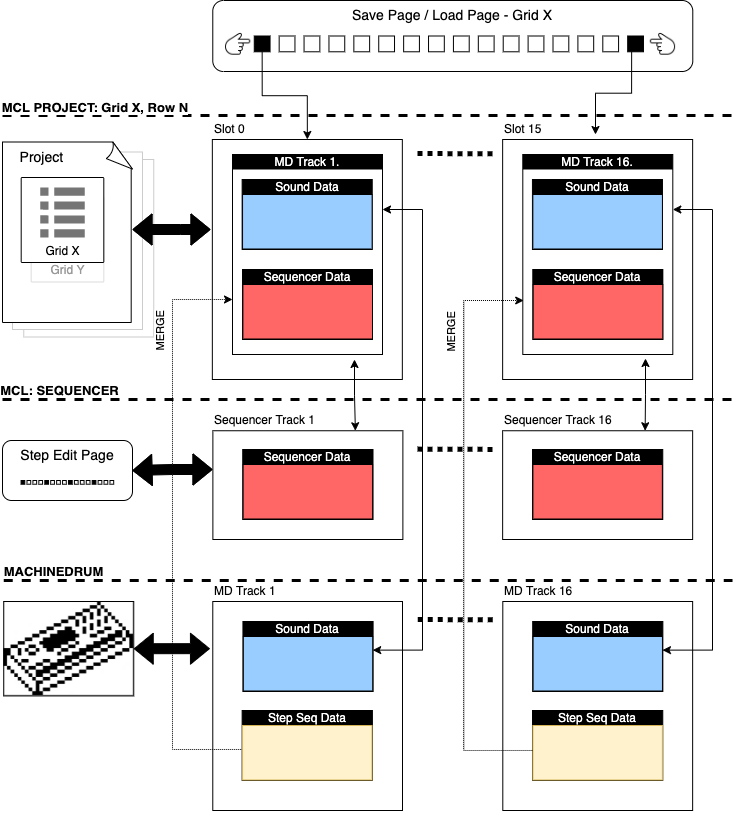
\includegraphics[scale=0.7]{save_or_load_grid_x.png}
    \caption{Save Page / Load Page - Grid X - MD }
    \label{fig:my_label}
\end{figure}
\begin{figure}
    \centering
    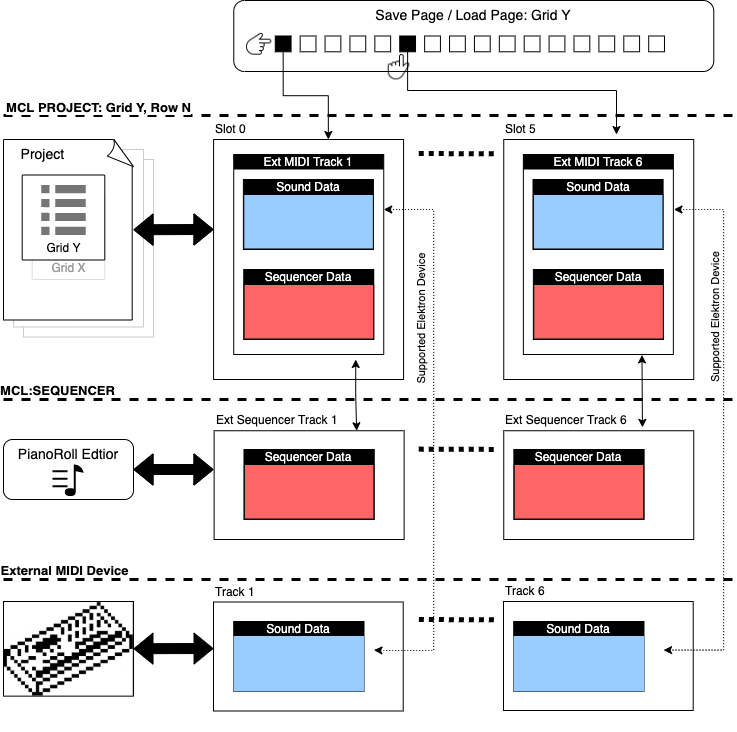
\includegraphics[scale=0.7]{save_or_load_grid_y.png}
    \caption{Save Page / Load Page - Grid Y - External MIDI}
    \label{fig:my_label}
\end{figure}
\begin{figure}
    \centering
    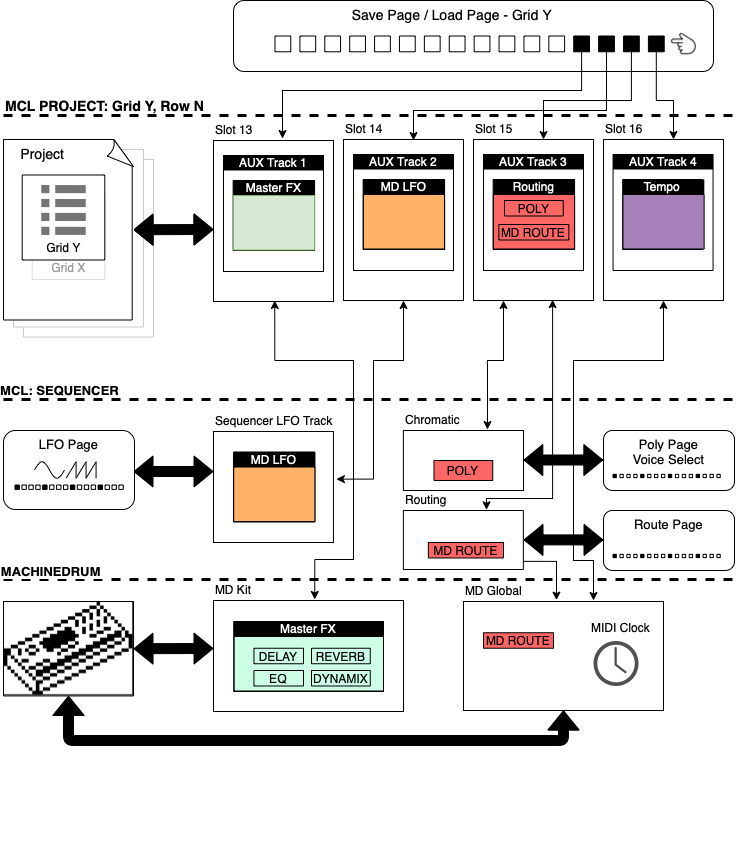
\includegraphics[scale=0.7]{save_or_load_grid_y_md.png}
    \caption{Save Page / Load Page - Grid Y - Auxiliary}
    \label{fig:my_label}
\end{figure}
